\section{Round Robin Implementation}

\subsection{Código}

En primer lugar, modificamos la declaracion de la clase  \texttt{SchedRR} agregando una serie de atributos privados:

\subsubsection{Class Declaration}
\begin{lstlisting}[language=C++, breaklines=true]
class SchedRR : public SchedBase {
	public:
		SchedRR(std::vector<int> argn);
        ~SchedRR();
		virtual void load(int pid);
		virtual void unblock(int pid);
		virtual int tick(int cpu, const enum Motivo m);

	private:
		int* quantum;
		int* cycles;
		std::queue<int> q;
};
\end{lstlisting}

Por un lado, el puntero de enteros llamado \texttt{quantum} nos dice por cuantos ciclos de clock nuestras tareas se van a ejecutar por CPU. Por otro lado, tenemos un puntero de enteros llamado \texttt{cycles}, que lo que hace es mantener la cuenta de cuantos ciclos le quedan a cada tarea en ejecución por CPU antes de llegar al quantum. Finalmente, tenemos una cola de tareas \texttt{q} compartida entre CPUs.

\subsubsection{Constructor y Destructor}
\begin{lstlisting}[language=C++, breaklines=true]
SchedRR::SchedRR(vector<int> argn) {
	// Round robin recibe la cantidad de cores y sus cpu_quantum por parametro
	quantum = new int[argn.size()-1];

	for (int i = 1; i < (int) argn.size(); i++) {
		quantum[i-1] = argn[i];
	}

	cycles = new int[argn[0]];
}
\end{lstlisting}

Aqui tenemos en \texttt{quantum} el arreglo del quantum por CPU, mientras que en \texttt{cycles} tenemos un arreglo que mantiene la cantidad de ciclos restantes del quantum de cada CPU.

\begin{lstlisting}[language=C++, breaklines=true]
SchedRR::~SchedRR() {
	delete[] cycles;
	delete[] quantum;
}
\end{lstlisting}

El destructor se encarga de liberar la memoria alocada por los dos arreglos.

\subsection{Load y Unblock}

\begin{lstlisting}[language=C++, breaklines=true]
void SchedRR::load(int pid) {
	q.push(pid);
}

void SchedRR::unblock(int pid) {
	q.push(pid);
}
\end{lstlisting}

Estas funciones se encargan de cargar tareas y de volverlas a cargar cuando se desbloquean. En este caso la implementacion es simple, ya que la migracion de procesos entre CPUs nos permite tener una unica cola, con lo cual alcanza con agregarlas a la misma para que entren en la rotacion de tareas.

\subsubsection{Tick}

Aqui tenemos el ciclo de ejecucion del $tick$ del scheduler, el mismo se encarga de manejar el desalojo de tareas:

\begin{lstlisting}[language=C++, breaklines=true]
int SchedRR::tick(int cpu, const enum Motivo m) {
	if (m == EXIT || m == BLOCK) {
		// Si el pid actual termino, sigue el proximo.
		if (q.empty()) return IDLE_TASK;
		else {
			int sig = q.front(); q.pop();
			cycles[cpu] = quantum[cpu];
			return sig;
		}
	} else {
		if (current_pid(cpu) == IDLE_TASK && !q.empty()) {
			int sig = q.front(); q.pop();
			cycles[cpu] = quantum[cpu];
			return sig;
		} else {
			cycles[cpu]--;

			if (cycles[cpu] == 0) {
				if (q.empty()) {
					cycles[cpu] = quantum[cpu];
					return current_pid(cpu);
				} else {
					int sig = q.front(); q.pop();
					q.push(current_pid(cpu)); // re-add to queue
					cycles[cpu] = quantum[cpu];
					return sig;
				}
			} else {
				return current_pid(cpu);
			}
		}
	}
}
\end{lstlisting}

Como podemos apreciar, primero se considera si la tarea actual ejecutandose en la CPU termino u ocurrio un bloqueo, en ambos casos se la desaloja y se la cambia por la siguiente tarea en la cola, resetando el quantum en el proceso. Si el procesador se encuantra ejecutando la tarea IDLE y hay tareas esperando a ser ejecutadas, se procede a ejecutar la primera que este en la cola y se resetea el quantum para la CPU. Si no se presentan ninguno de los dos casos anteriores, el scheduler chequea el quantum actual, si aun no termino se mantiene la tarea actual y se concluye el $tick$. En el caso que haya terminado el quantum se chequea la cola de tareas, si no hay tareas en espera se resetea el quantum, en el caso contrario se efectua el cambio de tarea con la primer tarea de la cola tambien reseteando el quantum.
\\
Para verificar la correcta implementacion de los mecanismos de $Round Robin$, tenemos la siguiente configuracion del scheduler:

\begin{enumerate}
	\item lote\_tsk: 2.tsk
	\item num\_cores: 2
	\item switch\_cost: 2
	\item sched\_class: SchedRR
	\item params: 5 10
\end{enumerate}

Esta configuracion fue usada durante el procesamiento del lote 4, que compone las siguientes tareas:

\begin{itemize}
	\item Tarea 0: 40 ciclos de CPU, 0 llamadas bloqueantes
	\item Tarea 1: 40 ciclos de CPU, 0 llamadas bloqueantes
	\item Tarea 2: 40 ciclos de CPU, 0 llamadas bloqueantes
	\item Tarea 3: 20 ciclos de CPU, 5 llamadas bloqueates, incorporada en el momento 10
\end{itemize}

El resultado obtenido fue el siguiente:

\begin{figure}[h]
    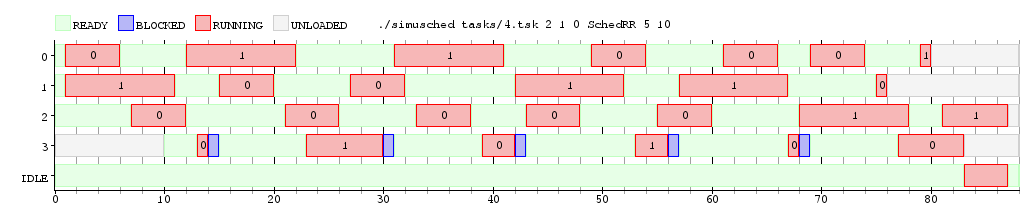
\includegraphics[width=\linewidth]{images/4.png}
    \label{fig:Task Consola}
    \caption{Task Batch}
\end{figure}

Como podemos apreciar en el grafico, cada uno de los \textit{Cores} tiene su propio quantum (5 y 10), por lo que el Round-Robin conmuta las tareas con distinta frecuencia según de que \textit{Core} se trate, no obstante la cola de espera (del estado \textit{ready}) es única, independientemente de la cantidad de \textit{Cores} (ambos tienen la misma cola). Debido a estas condiciones, dos tareas de tipo \textit{taskCPU} son ejecutadas al mismo tiempo (una en cada \textit{Core}), pero una es desalojada antes que la otra, suscitando a una operación de \textit{pop} en la cola y poniendo a la siguiente tarea en estado \textit{runing} bajo el \textit{Core} recien liberado. Esto deja al otro \textit{Core} ejecutando aún la misma tarea, y asignandole otra luego de un tiempo mayor de demora. Luego a este último \textit{Core} se le asigna la tarea 0 (antes ejecutada por el otro), dejandole al otro \textit{Core} la tarea numero 3 (aún no ejecutada) encolada oportunamente para la siguiente conmutación. Siguiendo el curso del grafico, la tarea numero 3, al ser de tipo \textit{TaskBatch}, tras realizar alguna llamada bloqueante es desalojada y conmutada con otra tarea en estado \textit{ready}, aún cuando su \textit{quantum} no haya sido consumido. Bajo estos principios el lote sigue ejecutandose hasta que no queden mas tareas, tras lo que pasa al estado \textit{runing} la tarea \textit{IDLE}.

Vale aclarar que en el caso de que alguna tarea actualmente ejecutandose consuma su \textit{quantum} y no haya alguna otra en estado \textit{ready}, la actual sigue en estado \textit{runing} hasta ese entonces (o hasta que dicha tarea finalice). 



